% Options for packages loaded elsewhere
% Options for packages loaded elsewhere
\PassOptionsToPackage{unicode}{hyperref}
\PassOptionsToPackage{hyphens}{url}
\PassOptionsToPackage{dvipsnames,svgnames,x11names}{xcolor}
%
\documentclass[
  letterpaper,
  DIV=11,
  numbers=noendperiod,
  oneside]{scrartcl}
\usepackage{xcolor}
\usepackage[left=1in,marginparwidth=2.0666666666667in,textwidth=4.1333333333333in,marginparsep=0.3in]{geometry}
\usepackage{amsmath,amssymb}
\setcounter{secnumdepth}{-\maxdimen} % remove section numbering
\usepackage{iftex}
\ifPDFTeX
  \usepackage[T1]{fontenc}
  \usepackage[utf8]{inputenc}
  \usepackage{textcomp} % provide euro and other symbols
\else % if luatex or xetex
  \usepackage{unicode-math} % this also loads fontspec
  \defaultfontfeatures{Scale=MatchLowercase}
  \defaultfontfeatures[\rmfamily]{Ligatures=TeX,Scale=1}
\fi
\usepackage{lmodern}
\ifPDFTeX\else
  % xetex/luatex font selection
\fi
% Use upquote if available, for straight quotes in verbatim environments
\IfFileExists{upquote.sty}{\usepackage{upquote}}{}
\IfFileExists{microtype.sty}{% use microtype if available
  \usepackage[]{microtype}
  \UseMicrotypeSet[protrusion]{basicmath} % disable protrusion for tt fonts
}{}
\makeatletter
\@ifundefined{KOMAClassName}{% if non-KOMA class
  \IfFileExists{parskip.sty}{%
    \usepackage{parskip}
  }{% else
    \setlength{\parindent}{0pt}
    \setlength{\parskip}{6pt plus 2pt minus 1pt}}
}{% if KOMA class
  \KOMAoptions{parskip=half}}
\makeatother
% Make \paragraph and \subparagraph free-standing
\makeatletter
\ifx\paragraph\undefined\else
  \let\oldparagraph\paragraph
  \renewcommand{\paragraph}{
    \@ifstar
      \xxxParagraphStar
      \xxxParagraphNoStar
  }
  \newcommand{\xxxParagraphStar}[1]{\oldparagraph*{#1}\mbox{}}
  \newcommand{\xxxParagraphNoStar}[1]{\oldparagraph{#1}\mbox{}}
\fi
\ifx\subparagraph\undefined\else
  \let\oldsubparagraph\subparagraph
  \renewcommand{\subparagraph}{
    \@ifstar
      \xxxSubParagraphStar
      \xxxSubParagraphNoStar
  }
  \newcommand{\xxxSubParagraphStar}[1]{\oldsubparagraph*{#1}\mbox{}}
  \newcommand{\xxxSubParagraphNoStar}[1]{\oldsubparagraph{#1}\mbox{}}
\fi
\makeatother


\usepackage{longtable,booktabs,array}
\usepackage{calc} % for calculating minipage widths
% Correct order of tables after \paragraph or \subparagraph
\usepackage{etoolbox}
\makeatletter
\patchcmd\longtable{\par}{\if@noskipsec\mbox{}\fi\par}{}{}
\makeatother
% Allow footnotes in longtable head/foot
\IfFileExists{footnotehyper.sty}{\usepackage{footnotehyper}}{\usepackage{footnote}}
\makesavenoteenv{longtable}
\usepackage{graphicx}
\makeatletter
\newsavebox\pandoc@box
\newcommand*\pandocbounded[1]{% scales image to fit in text height/width
  \sbox\pandoc@box{#1}%
  \Gscale@div\@tempa{\textheight}{\dimexpr\ht\pandoc@box+\dp\pandoc@box\relax}%
  \Gscale@div\@tempb{\linewidth}{\wd\pandoc@box}%
  \ifdim\@tempb\p@<\@tempa\p@\let\@tempa\@tempb\fi% select the smaller of both
  \ifdim\@tempa\p@<\p@\scalebox{\@tempa}{\usebox\pandoc@box}%
  \else\usebox{\pandoc@box}%
  \fi%
}
% Set default figure placement to htbp
\def\fps@figure{htbp}
\makeatother





\setlength{\emergencystretch}{3em} % prevent overfull lines

\providecommand{\tightlist}{%
  \setlength{\itemsep}{0pt}\setlength{\parskip}{0pt}}



 


% load packages
\usepackage{geometry}
\usepackage{xcolor}
\usepackage{eso-pic}
\usepackage{fancyhdr}
\usepackage{sectsty}
\usepackage{fontspec}
\usepackage{titlesec}

%% Set page size with a wider right margin
\geometry{a4paper, total={170mm,257mm}, left=20mm, top=20mm, bottom=20mm, right=50mm}

%% Let's define some colours
\definecolor{light}{HTML}{E6E6FA}
\definecolor{highlight}{HTML}{800080}
\definecolor{dark}{HTML}{330033}

%% Let's add the border on the right hand side 
% \AddToShipoutPicture{% 
%     \AtPageLowerLeft{% 
%         \put(\LenToUnit{\dimexpr\paperwidth-3cm},0){% 
%             \color{light}\rule{3cm}{\LenToUnit\paperheight}%
%           }%
%      }%
%      % logo
%     \AtPageLowerLeft{% start the bar at the bottom right of the page
%         \put(\LenToUnit{\dimexpr\paperwidth-2.25cm},27.2cm){% move it to the top right
%             \color{light}\includegraphics[width=1.5cm]{_extensions/nrennie/PrettyPDF/logo.png}
%           }%
%      }%
% }

%% Style the page number
\fancypagestyle{mystyle}{
  \fancyhf{}
  \renewcommand\headrulewidth{0pt}
  \fancyfoot[R]{\thepage}
  \fancyfootoffset{3.5cm}
}
\setlength{\footskip}{20pt}

%% style the chapter/section fonts
\chapterfont{\color{dark}\fontsize{20}{16.8}\selectfont}
\sectionfont{\color{dark}\fontsize{20}{16.8}\selectfont}
\subsectionfont{\color{dark}\fontsize{14}{16.8}\selectfont}
\titleformat{\subsection}
  {\sffamily\Large\bfseries}{\thesection}{1em}{}[{\titlerule[0.8pt]}]
  
% left align title
\makeatletter
\renewcommand{\maketitle}{\bgroup\setlength{\parindent}{0pt}
\begin{flushleft}
  {\sffamily\huge\textbf{\MakeUppercase{\@title}}} \vspace{0.3cm} \newline
  {\Large {\@subtitle}} \newline
  \@author
\end{flushleft}\egroup
}
\makeatother

%% Use some custom fonts
\setsansfont{Ubuntu}[
    Path=_extensions/nrennie/PrettyPDF/Ubuntu/,
    Scale=0.9,
    Extension = .ttf,
    UprightFont=*-Regular,
    BoldFont=*-Bold,
    ItalicFont=*-Italic,
    ]

\setmainfont{Ubuntu}[
    Path=_extensions/nrennie/PrettyPDF/Ubuntu/,
    Scale=0.9,
    Extension = .ttf,
    UprightFont=*-Regular,
    BoldFont=*-Bold,
    ItalicFont=*-Italic,
    ]
\KOMAoption{captions}{tableheading}
\makeatletter
\@ifpackageloaded{caption}{}{\usepackage{caption}}
\AtBeginDocument{%
\ifdefined\contentsname
  \renewcommand*\contentsname{Table of contents}
\else
  \newcommand\contentsname{Table of contents}
\fi
\ifdefined\listfigurename
  \renewcommand*\listfigurename{List of Figures}
\else
  \newcommand\listfigurename{List of Figures}
\fi
\ifdefined\listtablename
  \renewcommand*\listtablename{List of Tables}
\else
  \newcommand\listtablename{List of Tables}
\fi
\ifdefined\figurename
  \renewcommand*\figurename{Figure}
\else
  \newcommand\figurename{Figure}
\fi
\ifdefined\tablename
  \renewcommand*\tablename{Table}
\else
  \newcommand\tablename{Table}
\fi
}
\@ifpackageloaded{float}{}{\usepackage{float}}
\floatstyle{ruled}
\@ifundefined{c@chapter}{\newfloat{codelisting}{h}{lop}}{\newfloat{codelisting}{h}{lop}[chapter]}
\floatname{codelisting}{Listing}
\newcommand*\listoflistings{\listof{codelisting}{List of Listings}}
\makeatother
\makeatletter
\makeatother
\makeatletter
\@ifpackageloaded{caption}{}{\usepackage{caption}}
\@ifpackageloaded{subcaption}{}{\usepackage{subcaption}}
\makeatother
\makeatletter
\@ifpackageloaded{tcolorbox}{}{\usepackage[skins,breakable]{tcolorbox}}
\makeatother
\makeatletter
\@ifundefined{shadecolor}{\definecolor{shadecolor}{rgb}{.97, .97, .97}}{}
\makeatother
\makeatletter
\@ifundefined{codebgcolor}{\definecolor{codebgcolor}{named}{light}}{}
\makeatother
\makeatletter
\ifdefined\Shaded\renewenvironment{Shaded}{\begin{tcolorbox}[sharp corners, colback={codebgcolor}, boxrule=0pt, enhanced, breakable, frame hidden]}{\end{tcolorbox}}\fi
\makeatother
\makeatletter
\@ifpackageloaded{sidenotes}{}{\usepackage{sidenotes}}
\@ifpackageloaded{marginnote}{}{\usepackage{marginnote}}
\makeatother
\usepackage{bookmark}
\IfFileExists{xurl.sty}{\usepackage{xurl}}{} % add URL line breaks if available
\urlstyle{same}
\hypersetup{
  colorlinks=true,
  linkcolor={highlight},
  filecolor={Maroon},
  citecolor={Blue},
  urlcolor={highlight},
  pdfcreator={LaTeX via pandoc}}


\author{}
\date{}
\begin{document}

\pagestyle{mystyle}


\section{W6: Aesthetics}\label{w6-aesthetics}

\pandocbounded{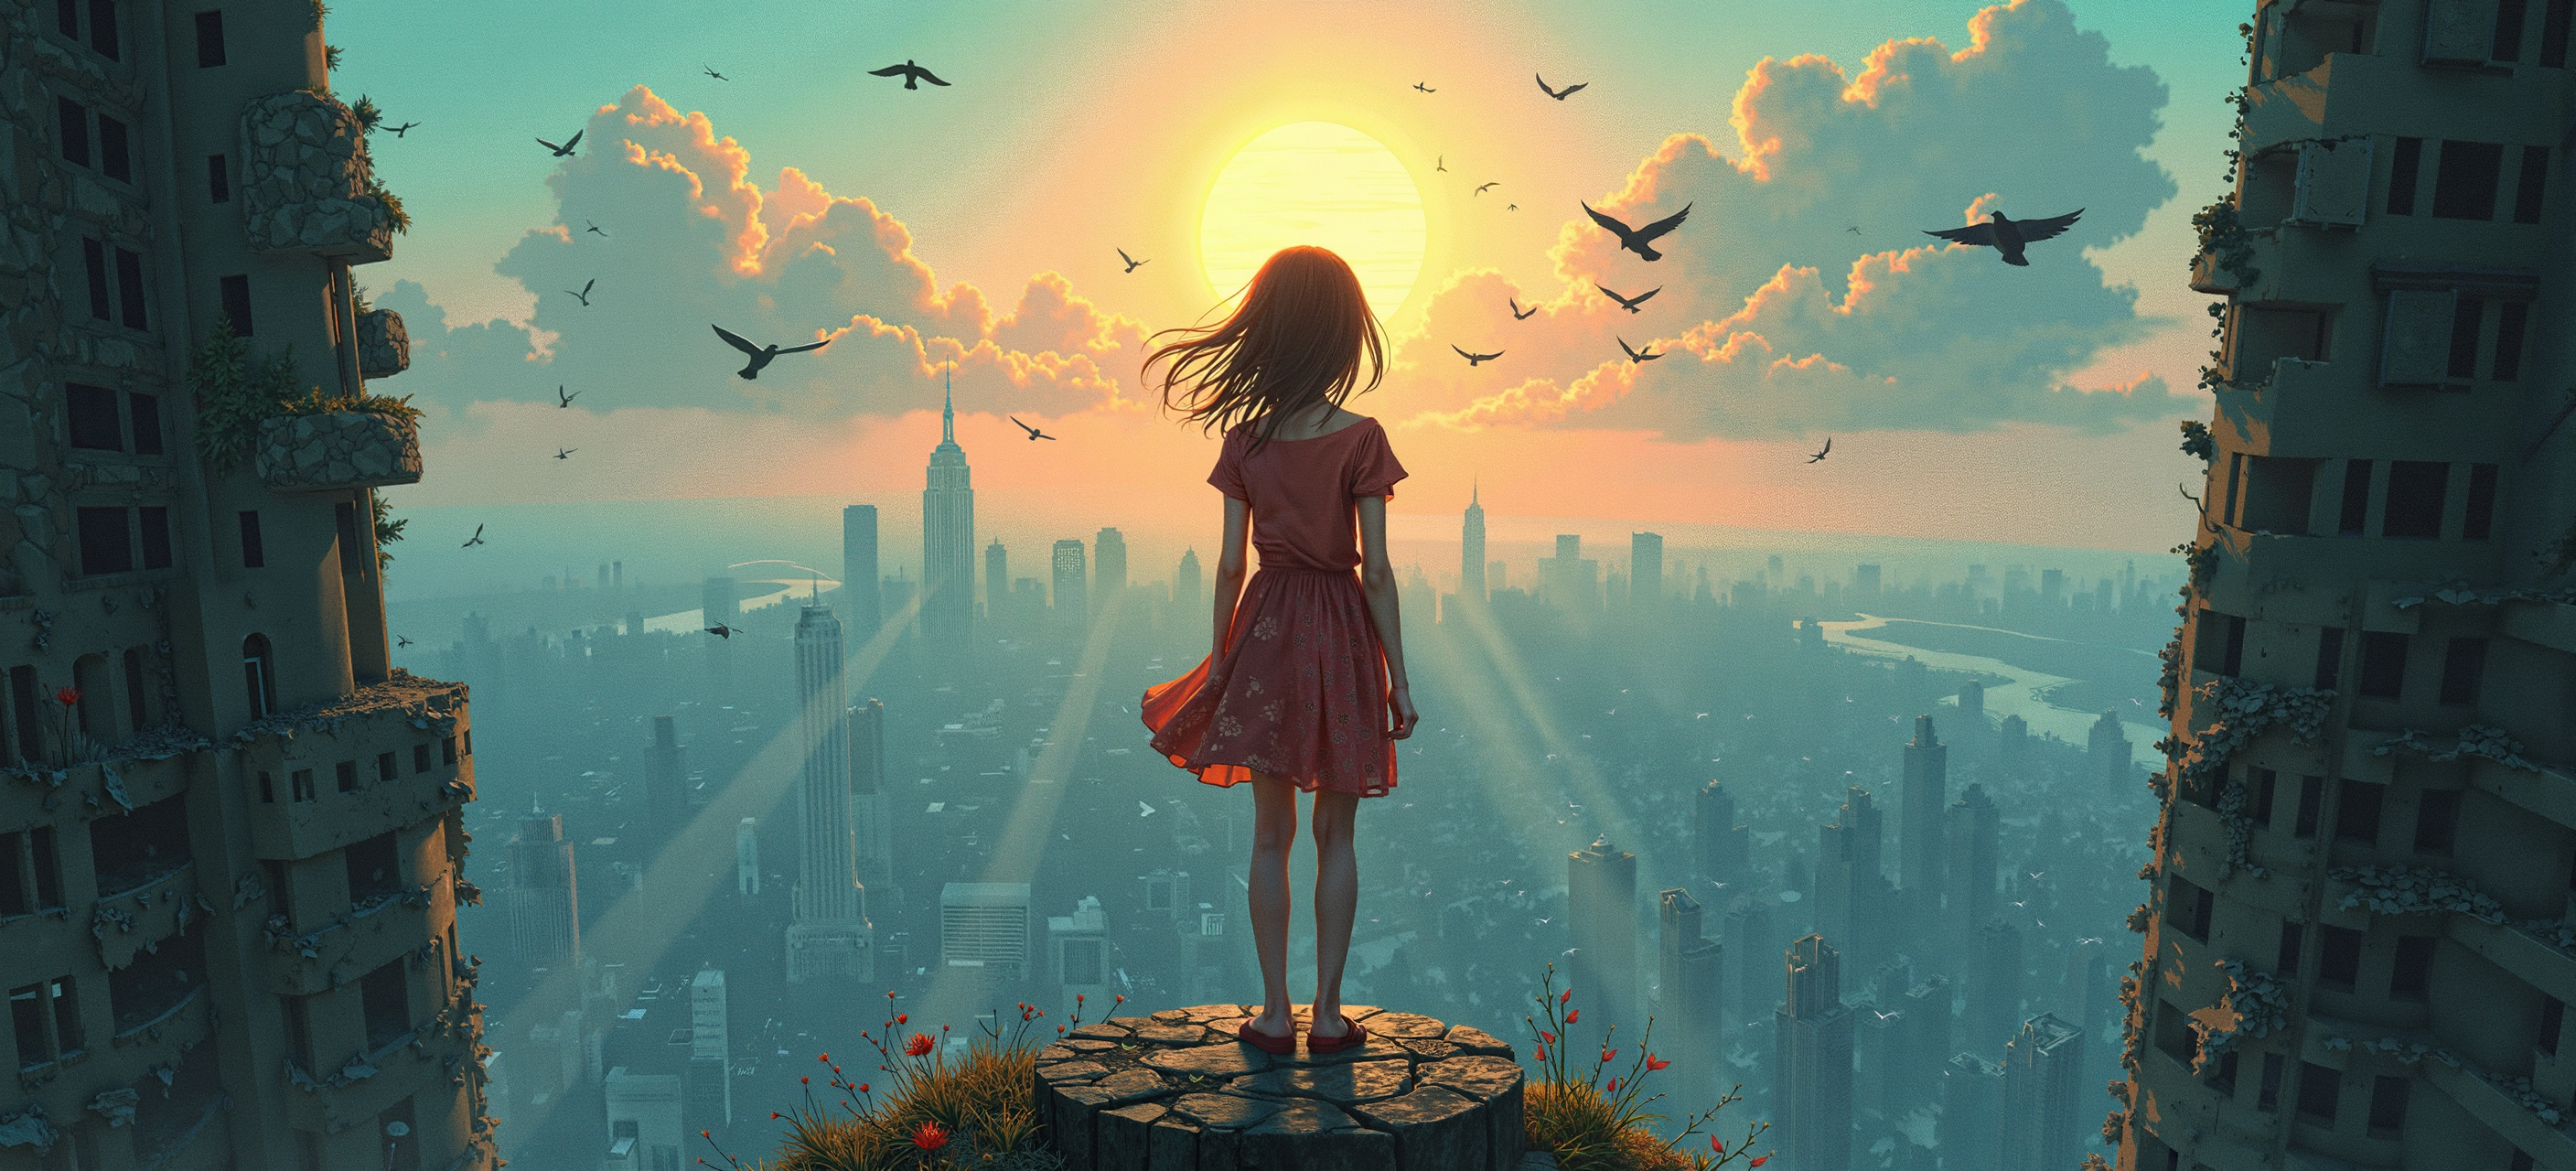
\includegraphics[keepaspectratio]{img/rgthree.png}}

\marginnote{\begin{footnotesize}

Guilherme Giolo and Michaël Berghman,
``\href{pdf/giolo-berghman-aesthetics.pdf}{The Aesthetics of the Self:
The Meaning-Making of Internet Aesthetics}''
\href{https://aesthetics.fandom.com/wiki/Aesthetics_Wiki}{Aesthetics
Wiki}

\end{footnotesize}}

What exactly \textbf{is} an ``aesthetic''? In what is to my knowledge
the only academic source to date to have explored the concept of the
aesthetic in theoretical terms,
\href{https://firstmonday.org/ojs/index.php/fm/article/view/12723}{Guilherme
Giolo and Michaël Berghman} (2023) suggest that traditional conceptual
frameworks such as genre, lifestyle, or subculture are no longer
adequate to understanding the contemporary modalities of cultural
identity and creativity. Instead, they explore the ubiquitous popular
concept of the ``aesthetic'' as the key component of a new analytical
framework. What does an ``aesthetic'' in this contemporary sense consist
of? We might start by examining the entry on
\href{https://aesthetics.fandom.com/wiki/City_Pop}{``City Pop''} on the
\href{https://aesthetics.fandom.com/wiki/Aesthetics_Wiki}{Aesthetics
Wiki}, a vast online catalogue of aesthetic styles from ``Algorave'' to
``Zombie Apocalyse'', ``Dark Academia'' to ``Visual-kei'',
``Cottagecore'' to ``Witch House''. Like many of the other entries about
aesthetics that the reader is already acquainted with, however, the city
pop entry, while a useful introduction, brings few surprises, opening
with a bland definition of it as ``a subgenre of Pop music from Japan''.
The remainder of the entry is a walkthrough of everything that everyone
at this conference already knows, with the obligatory references to
1970s American AOR, YMO, and the California Dreaming of Hiroshi Nagai.
What the entry doesn't get us much closer to, however, is understanding
why city pop can be considered not just as a J-pop subgenre but an
\textbf{aesthetic}. For that we need to go back to Giolo and Berghman.

\marginnote{\begin{footnotesize}

\href{https://aesthetics.fandom.com/wiki/City_Pop}{\includegraphics[width=1.04167in,height=\textheight,keepaspectratio]{img/plastic-love.webp}}

\end{footnotesize}}

One of the defining components of what Giolo and Berghman call Internet
aesthetics is their association with certain kinds of experience, and
the corresponding feelings evoked by the memory of that experience: the
experience of living in the world of 1950s America, for example, or the
world of Harry Potter; the experience of living in a dystopian future;
or, one might add, the experience of living on the American West Coast
in the 1970s, or in Tokyo at the height of the bubble economy. While
music is a key component of such experiences, it is only one modality
within a larger cultural world. Imaginatively speaking, aesthetics
recall the fantasy worlds of videogames and LARPing:

\begin{quote}
Experiences (and, likely, their importance for Internet aesthetics) seem
to be even more evident in the titles of playlists associated with
different aesthetics: ``You are studying in a haunted library with
ghosts'' (dark academia playlist), ``You found the entrance to a secret
garden'', ``You are falling for the protagonist in a fantasy novel''
(light royaltycore), or ``A playlist for old money living in the French
countryside'' (light academia). Even clearer here, multiple objects
(songs) are grouped and given symbolic meaning under a new interpretive
key. This key is experience-centered. Thus, it seems acceptable to
assume that experience is also the goal of an Internet aesthetic: to
become someone different, \emph{to feel as if living in a different
time} (2023) {[}Emphasis mine{]}
\end{quote}

The dominant musical modality of aesthetics is the \textbf{playlist},
and playlists can be thought of as scripts or catalysts for certain
kinds of experience: the dark cinematic vibe of \emph{film noir} in
jazz; chillout-room electronica; the moody self-absorption of shoegaze;
the entire ``After Hours'' DJ session collection. Although originating
in the album-based formats of the 1970s and 1980s, city pop today is
something that we \textbf{experience} as much as just listen to,
something that conjures up a particular \textbf{structure of feeling}
(as Raymond Williams used to call it); and the primary way we experience
it is through the playlist, whether in the form of the compilation
release (\textbf{Pacific Breeze}) or the endless-summer playlists of
YouTube and Spotify. With the advent of the playlist, all music became
background music---music \textbf{for} something, that creates the
ambience for certain kinds of experience: studying, barbecueing, driving
at night, lovemaking, being depressed after a breakup. Music has long
had this function, of course; its origins go back to the so-called
``mood music'' of the 1950s, when stereophonic recording began to turn
it into an environment: \textbf{Music For Lovers}; \textbf{Soothing
Sounds for Baby}; and several decades later, \textbf{Music For
Airports}. Since the 1990s, mood music has been replaced by the concept
of \textbf{vibe}, but both are arguably about music as a catalyst for
shared experience (or the imagination of such experience) and the
structures of feeling associated with them. It's no coincidence that the
current generation of city pop fans around the globe are too young to
have lived through the decades to which it provided the musical
soundtrack, since \textbf{anemoia}-----nostalgia for something one never
experienced directly-----is one of the key constituents of Internet
aesthetics. To listen to an album today such as Tatsurō Yamashita's
appropriately-titled \textbf{For You} (1982), most of us can only dream
of another, better time and place, when Japan was still surfing the
economic wave and the prevailing mood was for glamour and partying. A
decade later, after the bubble had burst, while Yasuharu Konishi's
Readymade Records continued to party like it was (not yet) 1999, the
vibe of Shibuya-kei led by Crue-el and Trattoria Records was cooler,
more circumspect, more indie---Music For The Morning After.

\marginnote{\begin{footnotesize}

\href{https://youtu.be/loSQDPUHazQ}{\includegraphics[width=1.04167in,height=\textheight,keepaspectratio]{img/for-you.jpg}}

\end{footnotesize}}

Giolo and Berghman also emphasize the affective dimension of Internet
aesthetics, and their interviewees frequently reference feelings when
describing them:

\begin{quote}
``The aesthetics that I like really depend on my mood of the day. On
Sundays, when it's sunny, I really enjoy aesthetic images that
\emph{give me this summer feeling}'' Jane (Dutch, prefers
``cottagecore'').

Jane, who strongly connects ``cottagecore'' to morning walks, went on to
explain that in those moments the scenarios and imaginaries of this
Internet aesthetic ``flow'' into her activity, representing ``the things
I would like at that moment. \emph{They give me a warming feeling}''
(2023). {[}Emphasis mine{]}
\end{quote}

By now we are (hopefully) getting closer to understanding what it means
to describe city pop as an aeesthetic rather than just a musical genre.
Like vaporwave, like future funk, like mallsoft, like lo-fi hip hop,
city pop conjures up a particular kind of cultural-historical aesthetic
experience and a corresponding affective structure, via playlists,
imagery, and other elements. As has been much discussed in the case of
vaporwave, the dominant temperamental register is nostalgic and
melancholic, invoking a bygone era of economic optimism and
technological utopianism rendered only more poignant by the harsh
realities of the dystopian present.




\end{document}
